\documentclass[a4paper,11pt]{article}

\usepackage[english]{babel}
\usepackage{mathrsfs, amssymb, amsmath, amsthm, enumerate}
\usepackage{verbatim,graphicx,geometry}
%\usetikzlibrary{arrows}
\usepackage[utf8]{inputenc}
\usepackage{authblk}
\usepackage[round]{natbib}
\bibliographystyle{plainnat}

\usepackage{hyperref}

\makeatletter
\def\@biblabel#1{\hspace*{-\labelsep}}
\makeatother
\geometry{left=1in,right=1
in,top=1in,bottom=1in}
\newdimen\dummy
\dummy=\oddsidemargin
\addtolength{\dummy}{72pt}
\marginparwidth=.5\dummy
\marginparsep=.1\dummy


\newcommand{\E}{\mathbb{E}}
\newcommand{\Var}{\mathrm{Var}}
\newcommand{\plim}{\overset{p}{\longrightarrow}}
\newcommand{\dlim}{\overset{d}{\longrightarrow}}

\begin{document}

\begin{table}
\centering
\begin{tabular}{llll}
\hline \hline
variable & value & objective function & interpretation \\ \hline
$\eta^H$ & 0.05 & 2.82 & New technology benefit \\
$\eta^M$ & 0.025 & 2.82 & New combination benefit \\
$\tau$ & 100 & 2.82 & Shape parameter for idea distribution \\
$\xi$ & 5 & 2.82 & $1/\xi$ is the fraction of viable combinations \\
$\lambda $ & 0.7 & 2.82 & scale parameter of the cost distribution \\
$\kappa $ & 3 & 2.82 & shape parameter of the cost distribution \\
\hline \hline
\end{tabular}
\caption{Current values that minimize the objective function}
\end{table}


\begin{table}
\centering
\begin{tabular}{llll}
\hline \hline
Column \# & Moment & Model & Data \\ \hline
1 & Fraction of refinements in 1880 & 28\% & 55\% \\
2 & Fraction of new combinations in 1880 & 65.5\% & 30\% \\
3 & Fraction of new technologies in 1880 & 6.46\% & 10\% \\
4 & Fraction of refinements in 1930 & 13.38\% & 35\% \\
5 & Fraction of new combinations in 1930 & 83.13\% & 60\% \\
6 & Fraction of new technologies in 1930 & 3.47\% & 3\% \\
7 & Peak of the refinement share & 60.95\% & 60\% \\
8 & Year of the peak in refinement share & 1846 & 1870 \\
\hline \hline
\end{tabular}
\caption{Moments}
\end{table}


\begin{figure}
\begin{center}
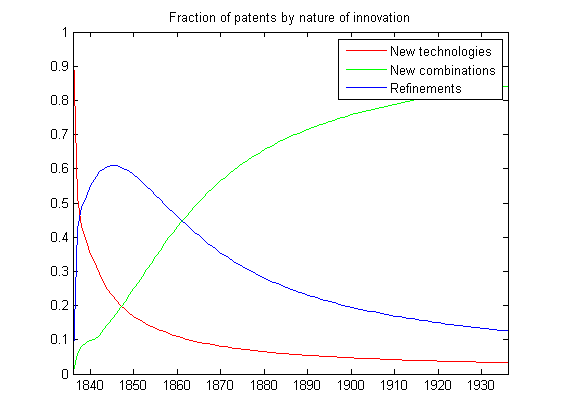
\includegraphics[scale=.8]{fractions2.png}
\caption{Fraction of patents by type}
\end{center}
\end{figure}


\end{document}